\chapter{Horizontes de de Sitter y probabilidad cosmológica}

\lectureoverview{Un horizonte no es simplemente una frontera causal. Para un observador estacionario es un sistema térmico: un termómetro situado a una distancia propia \(\rho\) del horizonte indica una temperatura del orden de \(1/(2\pi\rho)\), mientras que el corrimiento gravitatorio al rojo hace que la radiación observada a gran distancia sea mucho más fría. Aplicaremos esta lección sobre los agujeros negros al espacio de de Sitter, deduciremos el radio fijo del horizonte \(H^{-1}\) y escribiremos la métrica de la región estática del observador. La segunda mitad de la clase sigue las consecuencias inquietantes de la termodinámica: entropía finita de de Sitter, recurrencias de Poincaré, cerebros de Boltzmann, inflación eterna y el problema de la medida. Una última discusión distingue las estructuras supersimétricas exactas de la teoría de cuerdas del marco aún desconocido que quizá pueda describir nuestro mundo.}

\section{Qué significa que un horizonte esté caliente}

Comenzamos antes de la clase formal con la pregunta que marcará el rumbo de la sesión.

\begin{classroomqa}
\audiencequestion{Un horizonte cósmico no contiene ningún agujero negro. ¿Qué mecanismo puede, sin embargo, hacer que esté caliente?\lecturetimestamp{00:00:17}}
\lecturerresponse{El mecanismo es el mismo que en el caso de un horizonte de agujero negro. La pregunta útil es operacional: ¿qué registra un termómetro situado cerca del horizonte y qué radiación llega a un observador lejano?}
\end{classroomqa}

El primer experimento es local. Mantengamos un termómetro a una distancia propia fija \(\rho\) de cualquier horizonte suave y no extremo. Muy cerca del horizonte, la geometría adopta la forma universal de Rindler, y el termómetro indica
\begin{equation}
T_{\rm local}(\rho)\simeq \frac{1}{2\pi\rho}
\label{eq:l09-local-temperature}
\end{equation}
en unidades en las que \(\hbar=c=k_B=1\). Al restituir las constantes se obtiene
\begin{equation}
k_B T_{\rm local}(\rho)\simeq \frac{\hbar c}{2\pi\rho}.
\end{equation}
La divergencia cuando \(\rho\to0\) no significa que un observador en caída libre se encuentre con un horno material ordinario. Es la temperatura asignada por un observador que permanece estacionario justo fuera del horizonte y, por tanto, debe acelerarse cada vez más violentamente.

La conversación inicial también distingue tres conceptos que se confunden con facilidad: energía, temperatura y entropía.

\begin{classroomqa}
\audiencequestion{Si se envían fotones a un agujero negro, ¿seguimos midiendo la misma entropía o solo cambia la energía?\lecturetimestamp{00:01:22}}
\lecturerresponse{Cuando un fotón deja de ser accesible al quedar tras el horizonte, se ha ocultado información adicional. En el lenguaje simplificado de bits que usamos aquí, un fotón puede ocultar un bit adicional y, por tanto, aumentar la entropía. La energía, la temperatura y la entropía están relacionadas, pero no son intercambiables.}
\end{classroomqa}

\editorialnote{En un agujero negro físico, el cambio de entropía queda fijado termodinámicamente por \(dS=dE/T_H\); no es universalmente de un bit por cada fotón, con independencia de su energía. La afirmación de un bit es una idealización de teoría de la información empleada en la clase.}

La región cercana al horizonte emite y reabsorbe continuamente fluctuaciones cuánticas de alta frecuencia. Para el observador estacionario, el horizonte hace que esas fluctuaciones sean térmicas. Pero esto plantea de inmediato un enigma. Si la región está arbitrariamente caliente, ¿por qué un observador lejano no queda cegado por fotones de energía arbitrariamente alta?

\section{Corrimiento gravitatorio al rojo y temperatura de Hawking}

Una pared caliente ordinaria sigue siendo una fuente de radiación de alta frecuencia incluso cuando estamos lejos de ella. Un horizonte es distinto porque su radiación debe ascender a través de un corrimiento gravitatorio al rojo. La velocidad del fotón sigue siendo \(c\); lo que disminuye es su energía,
\begin{equation}
E=\hbar\omega,
\qquad
\omega_{\rm received}<\omega_{\rm emitted}.
\end{equation}
La analogía con un trozo de tiza lanzado, que se usa en la clase, solo es útil hasta aquí. Una piedra lanzada pierde velocidad al subir, mientras que un fotón sigue viajando a la velocidad de la luz, aunque disminuyan su frecuencia y su energía.

Para un agujero negro de Schwarzschild, la temperatura medida por un observador en el infinito es
\begin{equation}
T_H=\frac{1}{8\pi M}
\label{eq:l09-hawking-natural}
\end{equation}
en unidades \(G_N=\hbar=c=k_B=1\). En unidades ordinarias,
\begin{equation}
T_H=\frac{\hbar c^3}{8\pi G_N M k_B}.
\label{eq:l09-hawking-full}
\end{equation}

\begin{figure}[htbp]
\centering
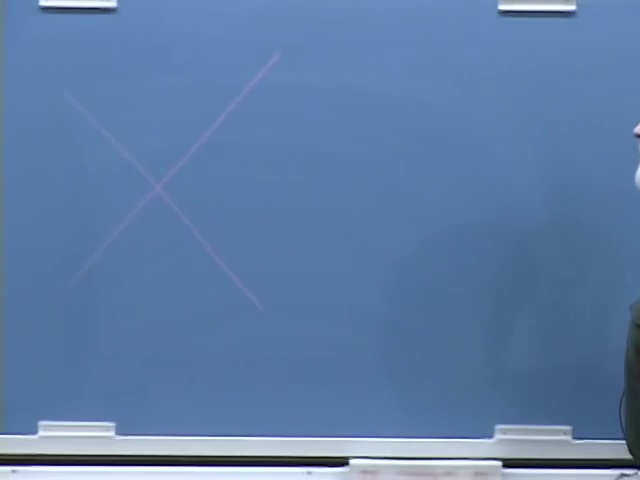
\includegraphics[width=0.68\textwidth]{lecture_09_figure_02.png}
\caption{La temperatura de Hawking \(T_H=1/(8\pi M)\) en unidades naturales.}
\lectureframe{00:08:12}
\end{figure}

Un agujero negro más grande es más frío. La clase lo explica siguiendo hacia atrás la trayectoria de un fotón típico. Los fotones térmicos tienen una energía característica \(E_\gamma\sim T_H\). Un fotón que llega al infinito con una energía del orden de \(M^{-1}\) tenía una energía local mucho mayor cuando se originó cerca del horizonte. El corrimiento al rojo entre la capa cercana al horizonte y el infinito es más intenso en un agujero más grande, por lo que la temperatura asintótica resultante es menor.

\begin{classroomqa}
\audiencequestion{Si el tiempo de Schwarzschild se congela en el horizonte, ¿deberíamos seguir el fotón que cayó originalmente y formó el agujero?\lecturetimestamp{00:04:19}}
\lecturerresponse{Para responder a la pregunta sobre la temperatura, sigamos los fotones emitidos hacia afuera. Se originan con una frecuencia local muy alta, pierden energía al ascender y llegan como radiación de Hawking. El destino del fotón que cayó originalmente es una cuestión distinta, relacionada con la información.}
\end{classroomqa}

\section{La capa de Planck y el horizonte estirado}

¿Hasta qué distancia del horizonte puede confiarse en la relación local de la ecuación~\eqref{eq:l09-local-temperature}? La clase toma la longitud de Planck como la distancia mínima con significado en la descripción semiclásica. Esto sugiere una capa delgada, situada aproximadamente a una longitud de Planck por fuera del horizonte matemático y llena de fluctuaciones a escala de Planck. Emite y absorbe continuamente.

La mayoría de los cuantos emitidos no escapan. Solo los que se dirigen dentro de un cono saliente muy estrecho evitan caer de nuevo. Los cuantos emitidos en direcciones genéricas regresan al horizonte. Las excitaciones salientes y entrantes chocan y producen pares y otras partículas; en este sentido, la descripción estacionaria contiene una capa delgada de material extremadamente caliente.

\begin{figure}[htbp]
\centering
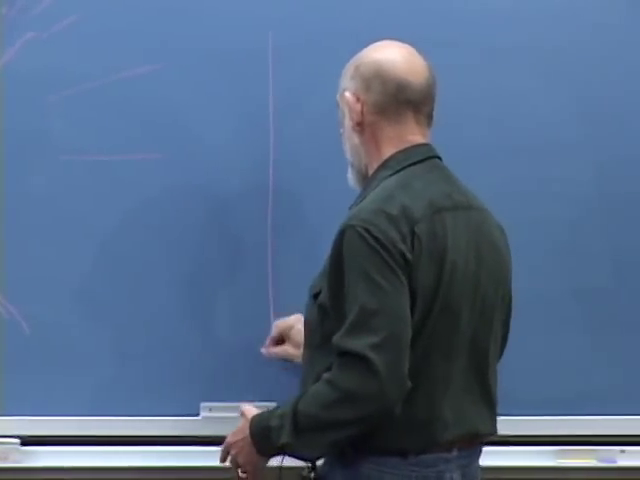
\includegraphics[width=0.74\textwidth]{lecture_09_figure_03.png}
\caption{El estrecho cono de escape de la radiación cercana al horizonte. La mayoría de los cuantos emitidos localmente regresa al horizonte.}
\lectureframe{00:11:38}
\end{figure}

Hay una imagen complementaria del espacio-tiempo. Lejos de un horizonte, una fluctuación virtual puede representarse esquemáticamente mediante un pequeño lazo cerrado: aparece y desaparece una excitación partícula-antipartícula antes de que pueda convertirse en un estado asintótico. Cerca de un horizonte, una fluctuación puede atravesar la frontera causal. Para el observador exterior, la parte que queda fuera parece una partícula emitida por el horizonte y reabsorbida más tarde. Una fracción muy pequeña escapa y se convierte en radiación de Hawking.

\begin{classroomqa}
\audiencequestion{En el diagrama exterior, ¿se extiende una fluctuación de ese tipo desde \(t=-\infty\) hasta \(t=+\infty\)?\lecturetimestamp{00:15:00}}
\lecturerresponse{El horizonte clásico exacto conduce a esa descripción de aspecto singular. En la práctica, lo sustituimos por un horizonte estirado: una superficie temporal situada aproximadamente a una longitud de Planck por fuera. Así, la emisión y la reabsorción ocurren en tiempos exteriores finitos.}
\end{classroomqa}

\begin{figure}[htbp]
\centering
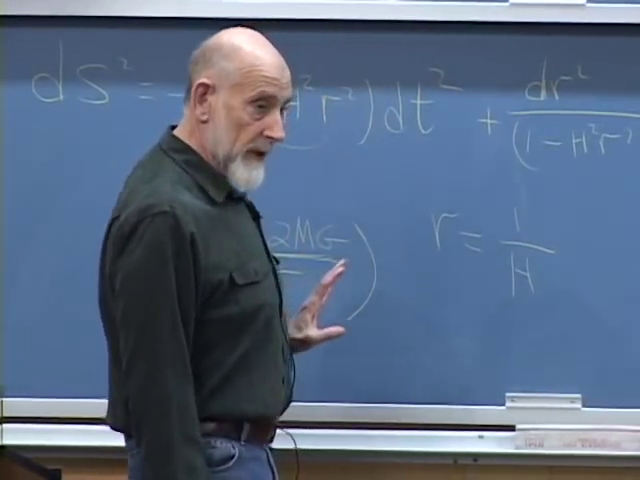
\includegraphics[width=0.72\textwidth]{lecture_09_figure_04.png}
\caption{El horizonte clásico y el horizonte estirado cercano que se usa en la descripción exterior.}
\lectureframe{00:15:52}
\end{figure}

El horizonte estirado no es una nueva frontera invariante. Es una superficie efectiva ubicada donde la geometría semiclásica deja de ser fiable. Las fluctuaciones cuánticas de la materia y de la propia geometría difuminan su ubicación exacta a escalas de Planck. Esta construcción representa esa incertidumbre mediante una superficie en la que la descripción exterior sigue siendo finita.

Nada en este argumento local permite saber si el horizonte pertenece a un agujero negro o a un universo en aceleración. Ese es el puente hacia el espacio de de Sitter.

\section{El espacio de de Sitter en coordenadas de expansión}

La clase formal comienza con la foliación espacialmente plana del espacio-tiempo de de Sitter,
\begin{equation}
ds^2=-dt^2+e^{2Ht}d\mathbf{x}^2,
\qquad
d\mathbf{x}^2=dx^2+dy^2+dz^2.
\label{eq:l09-flat-slicing}
\end{equation}
La constante \(H\) es la tasa de expansión de de Sitter. El factor aparece como \(e^{2Ht}\) porque la métrica mide distancias al cuadrado; un intervalo fijo en las coordenadas tiene una longitud física
\begin{equation}
D(t)=e^{Ht}\lvert\Delta\mathbf{x}\rvert.
\end{equation}

\begin{figure}[htbp]
\centering
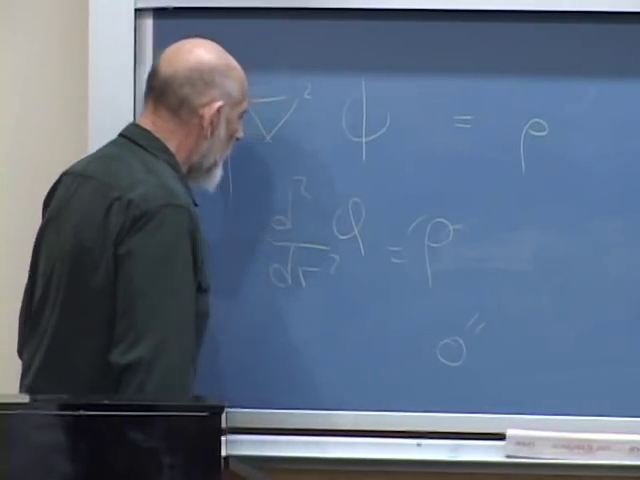
\includegraphics[width=0.78\textwidth]{lecture_09_figure_05.png}
\caption{La métrica de de Sitter, en expansión exponencial y coordenadas planas.}
\lectureframe{00:18:50}
\end{figure}

Estas coordenadas hacen evidente la expansión, pero sitúan el infinito futuro a una distancia infinita hacia arriba en la página. Para llevarlo a la pizarra, introduzcamos el tiempo conforme
\begin{equation}
\eta=-\frac{1}{H}e^{-Ht},
\qquad
-\infty<\eta<0.
\label{eq:l09-conformal-time}
\end{equation}
Entonces
\begin{equation}
dt=\frac{d\eta}{-H\eta},
\qquad
e^{Ht}=-\frac{1}{H\eta},
\end{equation}
y la ecuación~\eqref{eq:l09-flat-slicing} se convierte en
\begin{equation}
ds^2=\frac{1}{H^2\eta^2}
\left(-d\eta^2+d\mathbf{x}^2\right).
\label{eq:l09-conformal-metric}
\end{equation}
Cuando \(t\to+\infty\), \(\eta\to0^{-}\). El tiempo propio infinito se ha comprimido en la línea horizontal finita \(\eta=0\).

\editorialnote{La transformación temporal se corrige varias veces mientras se escribe en la pizarra. La ecuación~\eqref{eq:l09-conformal-time} es la forma coherente: los primeros tiempos cósmicos corresponden a \(\eta\to-\infty\) y el infinito futuro, a \(\eta\to0^{-}\).}

\begin{figure}[htbp]
\centering
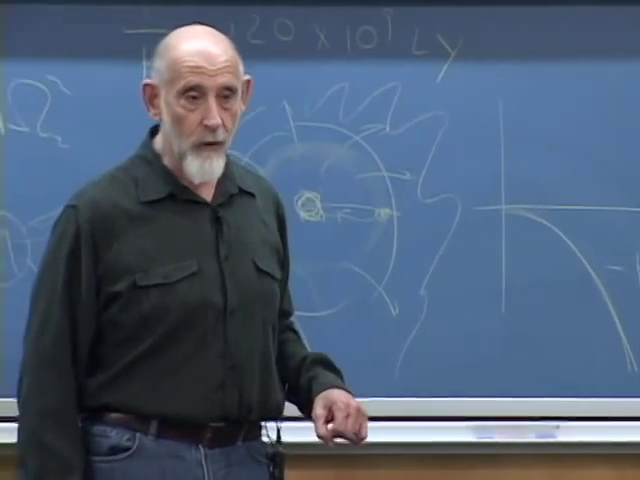
\includegraphics[width=0.82\textwidth]{lecture_09_figure_06.png}
\caption{La transformación al tiempo conforme y la métrica conforme plana.}
\lectureframe{00:21:24}
\end{figure}

El factor conforme multiplica tanto el término temporal como los espaciales, por lo que no altera las direcciones nulas. Para un rayo de luz radial,
\begin{equation}
ds^2=0
\quad\Longrightarrow\quad
-d\eta^2+dx^2=0
\quad\Longrightarrow\quad
\frac{dx}{d\eta}=\pm1.
\label{eq:l09-null-rays}
\end{equation}
Por tanto, la luz viaja a \(45^\circ\) en el diagrama conforme. Por eso resulta útil este cambio de coordenadas: permite visualizar la accesibilidad causal.

\section{La región causal de un observador}

Imaginemos un observador cuya línea de universo continúa durante un tiempo propio infinito. En el diagrama compactificado, termina en un punto de \(\eta=0\). Toda señal que el observador pueda recibir está dentro del cono de luz pasado de ese punto. Los sucesos fuera del cono nunca podrán comunicarse con el observador, por mucho que espere.

\begin{figure}[htbp]
\centering
\includegraphics[width=0.78\textwidth]{lecture_09_figure_07.png}
\caption{El cono de luz pasado límite de un observador en coordenadas conformes de de Sitter.}
\lectureframe{00:24:38}
\end{figure}

Un segundo observador tiene un cono distinto. Las dos regiones accesibles se solapan, pero ninguna abarca todo el espacio-tiempo. Para el resto del argumento, adoptaremos el punto de vista del primer observador y llamaremos región causal del observador a ese cono de luz pasado.

El dibujo parece mostrar cómo la región se contrae hacia el futuro, pero la anchura en coordenadas no es una distancia propia. En una hipersuperficie de \(\eta\), la distancia física al cuadrado entre el observador en \(x=0\) y el horizonte en \(x=\Delta x\) es
\begin{equation}
D^2=\frac{(\Delta x)^2}{H^2\eta^2}.
\label{eq:l09-horizon-distance-start}
\end{equation}
El horizonte es una línea nula a \(45^\circ\) que termina en \(\eta=0\); por tanto,
\begin{equation}
\Delta x=\lvert\eta\rvert.
\end{equation}
Al sustituir se obtiene
\begin{equation}
D_{\rm hor}^2=\frac{1}{H^2},
\qquad
D_{\rm hor}=\frac{1}{H}.
\label{eq:l09-horizon-radius}
\end{equation}
La separación en coordenadas disminuye, pero el factor conforme crece exactamente lo necesario para compensarla. El radio propio del horizonte es constante.

\begin{figure}[htbp]
\centering
\includegraphics[width=0.80\textwidth]{lecture_09_figure_08.png}
\caption{La derivación en la pizarra que convierte el intervalo decreciente en coordenadas en la distancia propia fija \(H^{-1}\).}
\lectureframe{00:28:42}
\end{figure}

\section{La región estática}

Un radio fijo del horizonte sugiere el uso de coordenadas adaptadas al observador central. Sin derivar la transformación de coordenadas, la clase escribe el resultado:
\begin{equation}
ds^2=
-\left(1-H^2r^2\right)d\tau^2
+\frac{dr^2}{1-H^2r^2}
+r^2d\Omega_2^2.
\label{eq:l09-static-patch}
\end{equation}
Los coeficientes dependen de \(r\), no de \(\tau\). Esta carta cubre la región estática del observador,
\begin{equation}
0\le r<\frac{1}{H}.
\end{equation}

\begin{figure}[htbp]
\centering
\includegraphics[width=0.88\textwidth]{lecture_09_figure_09.png}
\caption{La métrica de la región estática de de Sitter y su comparación con el factor de Schwarzschild.}
\lectureframe{00:34:22}
\end{figure}

El parecido con Schwarzschild es inmediato:
\begin{equation}
f_{\rm dS}(r)=1-H^2r^2,
\qquad
f_{\rm Schw}(r)=1-\frac{2G_NM}{r}.
\end{equation}
En ambos casos, el horizonte de las coordenadas estáticas se encuentra donde \(f(r)=0\). Para de Sitter,
\begin{equation}
1-H^2r^2=0
\quad\Longrightarrow\quad
r_H=H^{-1}.
\end{equation}
La carta es singular allí, igual que las coordenadas de Schwarzschild son singulares en el horizonte de un agujero negro. Sin embargo, las geometrías globales difieren en un aspecto importante. Un observador de un agujero negro está fuera y mira hacia dentro; un observador de de Sitter está dentro y mira hacia fuera.

\begin{classroomqa}
\audiencequestion{¿Cómo puede ser estática la geometría si las partículas en caída libre se alejan unas de otras en un universo que se expande exponencialmente?\lecturetimestamp{00:36:06}}
\lecturerresponse{Estático no significa que todas las partículas permanezcan inmóviles. Significa que los coeficientes de la métrica y el resultado de un experimento repetido son independientes del instante de inicio. Si soltamos dos partículas ahora, se aceleran alejándose; si repetimos el mismo experimento más tarde, ocurre el mismo movimiento.}
\end{classroomqa}

\begin{classroomqa}
\audiencequestion{¿Las dos partículas que se alejan la una de la otra se observan mutuamente con corrimiento al rojo?\lecturetimestamp{00:38:34}}
\lecturerresponse{Sí. El aumento de su separación produce un corrimiento al rojo relativo, aunque la métrica adaptada al observador sea independiente del tiempo.}
\end{classroomqa}

\section{La temperatura observada desde el interior}

Las estructuras cercanas al horizonte de Schwarzschild y al de de Sitter son localmente equivalentes. Por tanto, el horizonte de de Sitter emite y reabsorbe cuantos térmicos. Un fotón poco frecuente se propaga hacia el interior hasta el observador central y pierde energía al ascender por el potencial de la región estática. La temperatura de Gibbons--Hawking medida en el centro es
\begin{equation}
T_{\rm dS}=\frac{H}{2\pi}
\label{eq:l09-de-sitter-temperature}
\end{equation}
en unidades naturales. Un termómetro estacionario a un radio \(r\) indica el valor desplazado al rojo de Tolman
\begin{equation}
T_{\rm local}(r)=
\frac{T_{\rm dS}}{\sqrt{1-H^2r^2}},
\label{eq:l09-tolman}
\end{equation}
que diverge cuando \(r\to H^{-1}\) y se reduce, cerca del horizonte, a la ecuación~\eqref{eq:l09-local-temperature}.

\editorialnote{La clase obtiene la escala a partir de la distancia al horizonte y del corrimiento al rojo, en vez de escribir explícitamente las ecuaciones~\eqref{eq:l09-de-sitter-temperature} y \eqref{eq:l09-tolman}. Estas expresan la normalización estándar de ese argumento.}

Para la aceleración tardía observada, la clase emplea la estimación del período
\begin{equation}
H^{-1}\sim 20\times10^9\ {\rm light\ years}.
\label{eq:l09-lecture-horizon-estimate}
\end{equation}
Un fotón típico del horizonte tiene entonces una longitud de onda comparable a miles de millones de años luz. No se trata de radiación de fondo de microondas: es muchísimo más fría.

El experimento mental operacional consiste en una caña de pescar a escala cosmológica. Alicia permanece en \(r=0\), conecta un termómetro a una línea muy larga que también transmite datos y deja que la repulsión cósmica aleje el instrumento. Lo detiene justo antes del horizonte, espera a que vuelva la señal y detecta una temperatura local alta. El termómetro que tiene junto a ella, en el centro, indica el diminuto valor \(H/(2\pi)\). Un mismo horizonte permite ambas lecturas porque se realizan a potenciales gravitatorios distintos.

\section{Cruzar el horizonte}

La descripción clásica desde el exterior se parece a la conocida historia del agujero negro. Bob, situado en el centro, ve alejarse a Alicia. Sus señales sufren un corrimiento al rojo cada vez mayor y llegan cada vez más despacio; ella parece aplanarse contra el horizonte y finalmente se desvanece. Jane, una viajera que llega después, parece formar otra capa más delgada en un estrato sedimentario junto a la frontera.

\begin{classroomqa}
\audiencequestion{Desde nuestro punto de vista, ¿los objetos llegan a atravesar alguna vez el horizonte cósmico?\lecturetimestamp{00:45:30}}
\lecturerresponse{No en la descripción clásica del observador estático. Sus señales sufren un corrimiento al rojo y se desvanecen mientras su posición aparente se aproxima al horizonte. Sin embargo, en su propia descripción en caída libre, lo cruzan sin encontrar una superficie localmente singular.}
\end{classroomqa}

\begin{classroomqa}
\audiencequestion{¿El horizonte solo está caliente para los observadores que permanecen cerca sin cruzarlo? Una observadora en caída libre no se abrasa simplemente por atravesarlo, ¿verdad?\lecturetimestamp{00:48:27}}
\lecturerresponse{Alicia cruza suavemente el horizonte en su propio sistema de referencia. La temperatura extrema pertenece a la descripción estacionaria. Si Bob insiste en observar a Alicia cada vez más cerca del horizonte, tiene que iluminarla con longitudes de onda cada vez más cortas. El microscopio de Heisenberg que intenta usar deposita entonces suficiente energía para abrasar aquello que trata de observar.}
\end{classroomqa}

No hay contradicción entre dos sucesos locales. El observador estacionario y quien cae libre realizan mediciones radicalmente distintas. La complementariedad de horizontes plantea cómo pueden ser válidas ambas descripciones sin permitir que un observador compare directamente información duplicada.

\section{Un modelo newtoniano de la repulsión del vacío}

En este punto, un estudiante pregunta qué reemplaza el pozo gravitatorio del agujero negro. Susskind responde construyendo un modelo newtoniano. Sea \(\phi\) el potencial gravitatorio; la aceleración de una partícula de prueba es
\begin{equation}
\mathbf{a}=-\boldsymbol{\nabla}\phi.
\end{equation}
Para la materia ordinaria no relativista, la ecuación de Poisson es
\begin{equation}
\nabla^2\phi=4\pi G_N\rho.
\label{eq:l09-poisson}
\end{equation}

\begin{classroomqa}
\audiencequestion{Si los efectos del agujero negro se deben a su pozo gravitatorio, ¿cuál es la fuente correspondiente en el espacio de de Sitter?\lecturetimestamp{00:49:36}}
\lecturerresponse{La propia energía del vacío proporciona una fuente gravitatoria espacialmente uniforme. En una descripción newtoniana produce un potencial cuadrático, en lugar de un pozo \(1/r\).}
\end{classroomqa}

\begin{figure}[htbp]
\centering
\includegraphics[width=0.78\textwidth]{lecture_09_figure_10.png}
\caption{La ecuación de Poisson y la forma esquemática de la segunda derivada radial que se usa en la clase.}
\lectureframe{00:51:38}
\end{figure}

En la pizarra se omiten la normalización, los términos asociados a la medida esférica, la presión e incluso, al principio, el signo global, de modo que el ejercicio se reduce a
\begin{equation}
\frac{d^2\phi}{dr^2}\sim H^2.
\end{equation}
La deducción esencial es que una fuente constante da lugar a una función cuadrática. Con el signo necesario para la repulsión de de Sitter,
\begin{equation}
\phi_{\rm dS}(r)=-\frac{1}{2}H^2r^2,
\qquad
a_r=-\frac{d\phi_{\rm dS}}{dr}=H^2r.
\label{eq:l09-de-sitter-potential}
\end{equation}
La aceleración apunta hacia afuera y aumenta linealmente con la distancia. Al resolver \(\ddot r=H^2r\) se obtiene
\begin{equation}
r(\tau)=A e^{H\tau}+B e^{-H\tau},
\end{equation}
y la rama creciente reproduce así la separación exponencial.

\begin{figure}[htbp]
\centering
\includegraphics[width=0.76\textwidth]{lecture_09_figure_11.png}
\caption{La ecuación con fuente uniforme y el potencial cuadrático de de Sitter.}
\lectureframe{00:53:32}
\end{figure}

\editorialnote{En relatividad general, la aceleración en el campo débil de un fluido homogéneo depende de \(\rho+3p\), no solo de \(\rho\). La energía del vacío tiene \(p=-\rho\), de modo que \(\rho+3p=-2\rho\) y la aceleración es repulsiva. La ecuación~\eqref{eq:l09-de-sitter-potential} es el resultado de de Sitter con la normalización correcta; el cálculo en la pizarra sigue deliberadamente solo la dependencia cuadrática y el signo.}

Coloquemos una masa ordinaria \(M\) en el centro. El potencial cualitativo pasa a ser
\begin{equation}
\phi(r)=-\frac{G_NM}{r}-\frac{1}{2}H^2r^2,
\label{eq:l09-combined-potential}
\end{equation}
y la aceleración radial es
\begin{equation}
a_r=-\frac{G_NM}{r^2}+H^2r.
\end{equation}
A valores pequeños de \(r\) domina la atracción local; a valores grandes de \(r\) domina la repulsión del vacío. El equilibrio se produce en
\begin{equation}
r_\ast=\left(\frac{G_NM}{H^2}\right)^{1/3}.
\label{eq:l09-turnaround}
\end{equation}
Esta es la versión clara del máximo del potencial que presenta la clase. Explica cualitativamente por qué los sistemas ligados por la gravedad pueden permanecer unidos en las proximidades, mientras que las galaxias suficientemente lejanas se alejan con aceleración.

\begin{figure}[htbp]
\centering
\includegraphics[width=0.78\textwidth]{lecture_09_figure_12.png}
\caption{La atracción ordinaria \(1/r\) combinada con el potencial cuadrático invertido de de Sitter.}
\lectureframe{00:58:20}
\end{figure}

\begin{classroomqa}
\audiencequestion{¿Siguen siendo importantes las fuerzas ordinarias o la repulsión del vacío acabará desgarrando todas las agrupaciones de materia?\lecturetimestamp{00:57:29}}
\lecturerresponse{Hay que tener en cuenta todas las fuerzas. A escalas suficientemente pequeñas predominan la interacción electromagnética que mantiene unidos los sistemas y la gravedad local. La repulsión del vacío solo cobra importancia a distancias enormes, determinadas por \(H^{-1}\) y por la escala de equilibrio que corresponde a la masa ligada.}
\end{classroomqa}

\section{Una fuente, varios nombres}

La discusión se detiene ahora en la terminología. En el modelo que usamos, la energía del vacío, la constante cosmológica y la energía oscura no son tres sustancias aditivas. Son tres descripciones de la misma fuente \(w=-1\). Puede hablarse de un término constante en la ecuación de Einstein, de una densidad de energía del vacío invariante de Lorentz o del componente que impulsa la aceleración tardía.

\begin{classroomqa}
\audiencequestion{¿Están presentes a la vez la fuente newtoniana uniforme y la energía cuántica del vacío como efectos separados?\lecturetimestamp{00:59:14}}
\lecturerresponse{No. La densidad uniforme es el modelo newtoniano de esa misma fuente. En esta clase, energía del vacío, constante cosmológica y energía oscura se refieren a un único componente físico.}
\end{classroomqa}

\begin{classroomqa}
\audiencequestion{¿Tiene entonces el mismo fenómeno una descripción clásica y otra cuántica?\lecturetimestamp{01:00:32}}
\lecturerresponse{Su origen microscópico puede ser mecánico-cuántico, del mismo modo que parte de la masa del electrón tiene un origen cuántico. Una vez conocida la densidad de energía efectiva, esta entra en las ecuaciones clásicas de la gravedad como una fuente ordinaria. Desconocemos el origen último del valor observado.}
\end{classroomqa}

En unidades de Planck, la densidad de energía del vacío observada es extraordinariamente pequeña,
\begin{equation}
\rho_\Lambda\sim10^{-123}\rho_{\rm Pl},
\label{eq:l09-planck-smallness}
\end{equation}
hasta el factor convencional que se use para la densidad de Planck. Ese número tan pequeño constituye el problema de la constante cosmológica. También explica por qué el horizonte es tan grande: en cuatro dimensiones,
\begin{equation}
H^2=\frac{8\pi G_N}{3}\rho_\Lambda,
\qquad
r_H=H^{-1}.
\end{equation}
Si \(H\) fuera mayor, el horizonte sería menor, la temperatura central de de Sitter sería mayor y la aceleración repulsiva \(H^2r\) sería más intensa.

\begin{classroomqa}
\audiencequestion{¿Está relacionada la diminuta constante cosmológica con la constante de Planck y las fluctuaciones cuánticas?\lecturetimestamp{01:03:27}}
\lecturerresponse{La comparación más clara emplea unidades de Planck adimensionales, en las que \(G_N=\hbar=c=1\). En esas unidades, la densidad del vacío es unos \(123\) órdenes de magnitud menor que la densidad de Planck natural. Explicar esa jerarquía es uno de los problemas centrales de la física fundamental.}
\end{classroomqa}

\begin{classroomqa}
\audiencequestion{¿Tiene que ser la energía del vacío una constante cosmológica exactamente constante? ¿Podría disminuir el componente acelerado y acabar estabilizándose en cero?\lecturetimestamp{01:04:52}}
\lecturerresponse{Esa es una alternativa lógicamente posible: un campo dinámico de energía oscura podría variar con el tiempo. La clase adopta el caso constante porque las observaciones disponibles en aquel momento favorecían cada vez más un comportamiento cercano al de una constante cosmológica, no porque se hubiera demostrado imposible toda alternativa.}
\end{classroomqa}

\section{La astronomía en un futuro lejano}

En un universo que tiende asintóticamente al espacio de de Sitter, las estructuras que no están ligadas gravitatoriamente acaban cruzando el horizonte del observador. El fondo cósmico de microondas se desplaza al rojo hasta dejar de ser detectable. Las galaxias lejanas desaparecen. Un astrónomo que sobreviva quizá solo vea una agrupación gravitatoria local fusionada, dentro de una región por lo demás oscura.

\begin{classroomqa}
\audiencequestion{Sin telescopio, ¿alguien siquiera notaría que han desaparecido las galaxias lejanas?\lecturetimestamp{01:06:17}}
\lecturerresponse{Probablemente no. El problema de fondo es más profundo: incluso con instrumentos avanzados, quizá los observadores futuros carezcan de los trazadores distantes y del fondo de microondas que hoy nos permiten inferir la expansión.}
\end{classroomqa}

Entonces podría parecer convincente la antigua imagen de un universo de islas. La paradoja de Olbers no obligaría a llegar a otra conclusión, porque presupone una población infinita, estática y uniforme de fuentes luminosas; el observador del futuro solo vería las estrellas finitas de la agrupación local. La energía oscura no crea continuamente galaxias de reemplazo a partir del espacio vacío.

El horizonte del espacio de de Sitter exacto no se contrae alrededor de la galaxia local. Su radio físico permanece en \(H^{-1}\), un valor muchísimo mayor que el tamaño de una galaxia. Lo que desaparece es la materia no ligada que atraviesa esa frontera causal fija.

\begin{classroomqa}
\audiencequestion{¿Podrían las estrellas expulsadas de la galaxia servir como cuerpos de prueba para detectar la geometría a gran escala?\lecturetimestamp{01:11:25}}
\lecturerresponse{Durante un tiempo, sí. Los objetos expulsados y las señales luminosas de gran alcance podrían explorar la geometría. Pero el efecto solo se vuelve apreciable a distancias del orden de una fracción considerable de mil millones de años luz, por lo que el experimento requeriría tiempos cosmológicos.}
\end{classroomqa}

\begin{classroomqa}
\audiencequestion{¿Cómo sabemos que un horizonte lejano no nos ha ocultado ya la mayor parte del universo?\lecturetimestamp{01:11:45}}
\lecturerresponse{Ya vemos suficientes galaxias, corrimientos al rojo y radiación de fondo para medir la expansión y reconstruir la geometría a gran escala. Los observadores futuros privados de esos trazadores se enfrentarían a un problema de inferencia mucho más difícil.}
\end{classroomqa}

\begin{classroomqa}
\audiencequestion{Si el horizonte estuviera justo más allá de Andrómeda, ¿sería evidente su presencia?\lecturetimestamp{01:12:19}}
\lecturerresponse{Sí. Un horizonte tan pequeño requeriría un valor mucho mayor de \(H\), y la repulsión resultante alteraría considerablemente el movimiento de Andrómeda. El valor medido sitúa, en cambio, el horizonte asintótico a una escala inmensamente mayor.}
\end{classroomqa}

\begin{classroomqa}
\audiencequestion{¿Podrían estar ocurriendo nuevos Big Bangs más allá de nuestro horizonte?\lecturetimestamp{01:13:25}}
\lecturerresponse{Los sucesos que ocurren más allá del horizonte no son visibles para nosotros ni para nuestros descendientes. Más adelante en la clase se presentará una posibilidad relacionada, pero más precisa: la nucleación de burbujas en la inflación eterna.}
\end{classroomqa}

Con cohetes, relojes y varios miles de millones de años, los observadores futuros podrían enviar exploradores a través de una gran parte de la región y reconstruir su métrica. Sin embargo, en escalas de tiempo propias de un laboratorio o de una civilización, el efecto es casi inaccesible. Esta distinción corrige la afirmación excesiva de que sería imposible descubrir la expansión: está fuera del alcance práctico inmediato, pero no está prohibida en principio.

\begin{classroomqa}
\audiencequestion{¿Podrían los exploradores futuros determinar la geometría mucho antes de tener que esperar una recurrencia térmica?\lecturetimestamp{01:21:40}}
\lecturerresponse{Desde luego. No se propone medirla esperando una recurrencia. Los exploradores podrían cartografiar la región estática intercambiando señales luminosas a lo largo de distancias de miles de millones de años luz; tardarían muchísimo menos, aunque todavía necesitarían tiempos cosmológicos.}
\end{classroomqa}

\begin{classroomqa}
\audiencequestion{¿El corrimiento al rojo borraría toda la información que obtuvieran exploradores de ese tipo?\lecturetimestamp{01:23:24}}
\lecturerresponse{No, si exploran escalas muy inferiores al horizonte. Una línea de base del orden de mil millones de años luz ya es sensible a la expansión y produce solo un corrimiento al rojo moderado. El experimento está limitado, sobre todo, por su duración inmensa.}
\end{classroomqa}

\section{Entropía finita y recurrencia}

El parche estático no está vacío en sentido termodinámico. Su horizonte tiene un área
\begin{equation}
A_H=4\pi H^{-2},
\end{equation}
una temperatura \(T_{\rm dS}=H/(2\pi)\) y una entropía
\begin{equation}
S_{\rm dS}=\frac{A_H}{4G_N}
=\frac{\pi}{G_NH^2}
\label{eq:l09-de-sitter-entropy}
\end{equation}
en unidades \(\hbar=c=k_B=1\). La entropía es finita. Por tanto, con las debidas cautelas, se puede imaginar el parche estático como una cavidad térmica de entropía finita, cuyas excitaciones se concentran cerca del horizonte en la descripción estacionaria.

Una caja ordinaria de gas en equilibrio parece no tener estructura en escalas de tiempo cortas, pero la mecánica estadística no prohíbe las fluctuaciones. Si un macroestado tiene un déficit de entropía \(\Delta S\) respecto del equilibrio, su probabilidad es aproximadamente
\begin{equation}
P\sim e^{-\Delta S}.
\label{eq:l09-fluctuation-probability}
\end{equation}
El tiempo de espera correspondiente crece como
\begin{equation}
t\sim t_0 e^{\Delta S}.
\end{equation}
En un sistema finito, el tiempo necesario para volver a un estado arbitrariamente cercano a uno anterior es el tiempo de recurrencia de Poincaré,
\begin{equation}
t_{\rm rec}\sim H^{-1}e^{S_{\rm dS}}.
\label{eq:l09-recurrence}
\end{equation}
Como \(S_{\rm dS}\) de nuestro horizonte es del orden de \(10^{120}\), la clase resume la escala como \(e^{10^{120}}\). Es irrelevante si el prefactor se mide en años, tiempos de Hubble o unidades microscópicas, frente a la doble exponencial.

\begin{figure}[htbp]
\centering
\includegraphics[width=0.76\textwidth]{lecture_09_figure_13.png}
\caption{La discusión sobre recurrencia, con la enorme escala exponencial del tiempo de espera escrita en la pizarra.}
\lectureframe{01:16:24}
\end{figure}

Antes de una recurrencia semejante, las fluctuaciones menores son muchísimo más frecuentes. Todas las moléculas de una habitación podrían reunirse en una esquina; podría formarse brevemente un vórtice complicado; en la jerarquía jocosa de la clase, el movimiento térmico podría ensamblar un elefante. Cuanto menor sea el déficit de entropía requerido, menos costosa será la fluctuación.

\begin{classroomqa}
\audiencequestion{¿Las recurrencias de Poincaré son específicamente una consecuencia de la mecánica cuántica?\lecturetimestamp{01:25:44}}
\lecturerresponse{No. La recurrencia y las fluctuaciones raras ya aparecen en la mecánica estadística clásica. Su aplicación al espacio de de Sitter se basa en nuestro marco físico actual, que quizá algún día se revise, pero la termodinámica y el razonamiento estadístico se cuentan entre las estructuras más sólidas que conocemos.}
\end{classroomqa}

El significado mismo de la probabilidad podría profundizarse en una teoría futura. Susskind no afirma lo contrario. Su planteamiento, más acotado, es que abandonar la mecánica estadística solo porque sus implicaciones a largo plazo resultan extrañas supondría descartar uno de los principios organizadores mejor comprobados de la física.

\section{Cerebros de Boltzmann y observadores típicos}

Supongamos que una fluctuación térmica crea un estado entero semejante al big bang. Eso requiere una disminución enorme de la entropía. Una fluctuación que produzca un sistema solar cuesta menos; una que produzca una Tierra ya cálida, menos aún. Si el único requisito es que haya un observador, la fluctuación menos costosa quizá solo crearía un cerebro funcional con recuerdos aparentes. A ese observador hipotético se le llama cerebro de Boltzmann.

La cuestión no es si una fluctuación extravagante es lógicamente posible. La cuestión es si un modelo cosmológico predice que casi todos los observadores son fluctuaciones de ese tipo. Inferimos a partir de nuestras observaciones suponiendo que no somos extraordinariamente atípicos. Una teoría en la que los observadores ordinarios, con historias cósmicas coherentes, quedan superados exponencialmente en número por cerebros térmicos aislados socava esa inferencia.

Por tanto, el problema de los cerebros de Boltzmann plantea una prueba cuantitativa de consistencia. Se compara la abundancia esperada de observadores ordinarios con la de observadores surgidos de fluctuaciones. Si predominan estos últimos, habrá que concluir que el vacío debe decaer antes de que proliferen, que hay que cambiar la medida o que deben reconsiderarse los supuestos cosmológicos.

Se deja explícitamente para más adelante una pregunta anterior sobre una conexión entre el ultravioleta--el infrarrojo. El argumento de recurrencia no depende de resolver esa cuestión aparte.

\section{Inflación eterna y universos burbuja}

A continuación, la clase introduce un segundo problema de probabilidad, sin intentar derivarlo por completo. En un vacío metastable de de Sitter puede nuclearse una burbuja cuyo vacío tiene menor energía. La pared de la burbuja se expande y el interior puede evolucionar hasta convertirse en un universo de Friedmann--Robertson--Walker abierto. Mientras tanto, la región inflacionaria circundante sigue expandiéndose y nuclea más burbujas.

\begin{figure}[htbp]
\centering
\includegraphics[width=0.74\textwidth]{lecture_09_figure_14.png}
\caption{Una burbuja con menor energía del vacío dibujada dentro de un fondo de de Sitter en inflación.}
\lectureframe{01:29:38}
\end{figure}

La característica crucial es el crecimiento exponencial de la población. Se produce nuevo volumen físico más deprisa de lo que las burbujas lo eliminan, así que el número de regiones burbuja crece sin límite. Distintas burbujas pueden asentarse en estados de baja energía diferentes y, por tanto, presentar una física efectiva distinta.

Para exponer la dificultad estadística, Susskind deja primero la cosmología y considera una población humana en crecimiento exponencial con recursos finitos, pero desconocidos. Supongamos que los observadores son típicos entre todas las personas que llegarán a vivir. Si la población se duplica en cada generación y luego desaparece, la mitad de todas las personas vivirá en la última generación, tres cuartas partes en las dos últimas y siete octavas partes en las tres últimas:
\begin{equation}
f_n=1-2^{-n}.
\label{eq:l09-last-generations}
\end{equation}
La tipicidad nos situaría entonces incómodamente cerca del final, aunque no sepamos nada sobre la cantidad total de recursos. Esto no se ofrece como una predicción fiable de la extinción humana. Es una advertencia: el crecimiento exponencial hace que los recuentos estén dominados por el corte.

El ejemplo de quienes lanzan monedas expresa con más claridad la suposición habitual de tipicidad. Si muchos experimentadores lanzan cada uno una moneda equilibrada \(N\) veces, la inmensa mayoría obtiene
\begin{equation}
n_H=\frac{N}{2}+O(\sqrt{N}).
\end{equation}
Un observador con un resultado extremo debería sospechar primero que el modelo o la moneda son defectuosos, en vez de suponer sin pruebas que ocupa una cola extraordinariamente rara. La probabilidad cosmológica parte de la misma intuición sobre la tipicidad, pero en una población infinita necesita un método de recuento bien definido.

\section{El límite de Escher y el problema de la medida}

La analogía geométrica de Susskind es \ M.\ C.\emph{Circle Limit IV}, de Escher: el disco teselado con ángeles y demonios que parecen más pequeños al acercarse al borde. En la geometría hiperbólica representada por el dibujo, las figuras son equivalentes; su tamaño euclidiano aparente solo cambia debido a la proyección.

\begin{figure}[htbp]
\centering
\includegraphics[width=0.76\textwidth]{lecture_09_figure_15.png}
\caption{El sustituto en la pizarra de las figuras de Escher que proliferan exponencialmente cerca de un límite circular.}
\lectureframe{01:37:54}
\end{figure}

Imaginemos que Escher dispone de tiempo, tinta y paciencia finitos. Al acercarse al borde, acaba por detenerse, quizá dejando algunas figuras incompletas. Como el número de figuras crece exponencialmente con el radio hiperbólico, una capa exterior de grosor finito contiene una fracción fija de todas las figuras dibujadas. Aproximadamente la mitad puede quedar en la capa final, por lejos que se desplace hacia fuera el corte.

Preguntemos ahora por la proporción entre ángeles y demonios. En el patrón infinito ideal, la simetría sugiere una igualdad uno a uno. Sin embargo, en cualquier recuento finito, un límite ligeramente distinto puede incluir muchas más figuras de un tipo. Como la mayor parte del recuento se concentra cerca del límite, una pequeña deformación de este produce un cambio de orden uno en el resultado.

\begin{figure}[htbp]
\centering
\includegraphics[width=0.76\textwidth]{lecture_09_figure_16.png}
\caption{En un patrón de crecimiento exponencial, el límite de corte domina el recuento.}
\lectureframe{01:43:06}
\end{figure}

La misma ambigüedad aparece en la inflación eterna. Se cuentan los universos burbuja azules y rosas por debajo de cierto corte temporal y luego se desplaza el corte hacia tiempos posteriores. Ambos recuentos divergen, y su proporción puede depender mucho de qué significa \emph{tiempo} y de cómo se trace la superficie de corte. Una medida de probabilidad es una prescripción que regula la población infinita y extrae probabilidades relativas. Que distintas prescripciones plausibles no coincidan constituye el problema de la medida.

\begin{classroomqa}
\audiencequestion{¿Hay alguna relación entre este problema del corte y la renormalización?\lecturetimestamp{01:45:43}}
\lecturerresponse{Hay una analogía. En teoría cuántica de campos se introduce una retícula o un corte ultravioleta, se refina y se buscan magnitudes insensibles a los detalles del borde del regulador. Los cosmólogos esperan obtener una extracción igual de robusta de la inflación eterna, pero en el marco que se analiza aquí todavía no hay una prescripción de solidez comparable.}
\end{classroomqa}

No conviene llevar demasiado lejos la analogía. La renormalización funciona cuando un flujo controlado identifica observables independientes del regulador. El problema de la medida consiste precisamente en que no están claras las preguntas invariantes análogas ni el procedimiento límite. Decir que quizá estamos planteando la pregunta equivocada no resuelve nada mientras no se formule la pregunta correcta.

\begin{classroomqa}
\audiencequestion{¿Esta imagen de burbujas es el mismo fenómeno que la inflación de nuestro universo temprano?\lecturetimestamp{01:48:19}}
\lecturerresponse{Está estrechamente relacionada. En la inflación eterna, el fondo progenitor sigue inflándose mientras los interiores de las burbujas locales atraviesan su propia evolución cosmológica. Nuestro universo observable podría estar dentro de una región semejante.}
\end{classroomqa}

\section{¿Podrían observarse colisiones entre burbujas?}

Cuando dos burbujas se encuentran, sus energías del vacío no se suman sin más. Una pared de dominio separa regiones con distintos estados del vacío, y la geometría de la pared determina qué puede observar cada lado. Según dónde se produzca la colisión con respecto a nuestro cono de luz pasado, su huella podría quedar oculta o ser visible.

\begin{classroomqa}
\audiencequestion{¿Qué ocurre cuando colisionan dos burbujas de vacío?\lecturetimestamp{01:52:07}}
\lecturerresponse{La colisión genera una geometría de pared de dominio cuyo comportamiento depende de los dos vacíos y de la tensión de la pared. En circunstancias causales favorables, la perturbación puede entrar en nuestra región observable y dejar una señal anisótropa.}
\end{classroomqa}

La clase analiza una región fría del fondo cósmico de microondas como posible candidata y señala la polarización alrededor de una estructura circular como elemento discriminante. Se presenta deliberadamente como una posibilidad, no como una detección. Una señal convincente de una colisión sería revolucionaria, porque aportaría evidencia directa de regiones burbuja vecinas y haría urgente desde el punto de vista experimental el problema de la medida.

\begin{figure}[htbp]
\centering
\includegraphics[width=0.70\textwidth]{lecture_09_figure_17.png}
\caption{Una estructura circular en el cielo y su posible patrón de polarización en la discusión sobre colisiones de burbujas.}
\lectureframe{01:50:22}
\end{figure}

\editorialnote{La discusión sobre la mancha fría recoge el estado de las observaciones y las propuestas vigentes en el momento de la clase. Una anomalía de temperatura por sí sola no constituye evidencia de una colisión de burbujas; haría falta una señal detallada y correlacionada.}

\begin{classroomqa}
\audiencequestion{¿Las burbujas son tetradimensionales y qué curvatura espacial tienen sus interiores?\lecturetimestamp{01:53:37}}
\lecturerresponse{Son regiones del espacio-tiempo, no burbujas de jabón tridimensionales que evolucionan en un tiempo externo. Sus interiores suelen ser universos FRW abiertos con curvatura espacial negativa. Una colisión perturba esa geometría, pero no convierte sin más la curvatura negativa en positiva.}
\end{classroomqa}

\section{Qué establece la teoría de cuerdas y qué no}

La discusión final comienza con una invitación a asignar una probabilidad de que la teoría de cuerdas sea correcta. Susskind se niega a dar una cifra porque la proposición es demasiado ambigua. En su lugar, distingue dos afirmaciones.

En primer lugar, existe una estructura matemática muy restringida que combina la mecánica cuántica y la gravedad. Ha producido resultados precisos e identidades matemáticas profundas, y su consistencia interna ha resistido un examen exhaustivo. En el vocabulario informal de la clase, esto es \emph{la Teoría de Cuerdas} con mayúscula \(S\). Las versiones que mejor se comprenden dependen en gran medida de la supersimetría.

En segundo lugar, el mundo observado no es supersimétrico a las energías accesibles. Conectar las construcciones supersimétricas exactas con nuestro universo no supersimétrico requiere la ruptura de la supersimetría y un marco más amplio que no está controlado con la misma precisión. En el vocabulario de la clase, esa extensión esperada es \emph{la teoría de cuerdas} con minúscula \(s\).

\begin{classroomqa}
\audiencequestion{¿Se puede asignar una probabilidad de que la teoría de cuerdas sea la teoría correcta de la naturaleza?\lecturetimestamp{01:54:18}}
\lecturerresponse{No sería responsable hacerlo sin especificar a cuál de las afirmaciones nos referimos. Las estructuras matemáticas exactas existen e incluyen la gravedad cuántica, pero los modelos supersimétricos bajo control riguroso no son literalmente el mundo que observamos. Que una extensión más amplia contenga nuestro mundo es una cuestión sobre la que los físicos pueden tener opiniones informadas, pero no admite una probabilidad numérica bien definida.}
\end{classroomqa}

La analogía es con la mecánica, antes de que se dispusiera de todo el aparato matemático. Se podrían conocer \(F=ma\) y la fuerza inversamente proporcional al cuadrado de la distancia, pero solo ser capaz de resolver órbitas circulares con mucha simetría. El sector resoluble sería auténtico, pero no abarcaría toda la teoría. Del mismo modo, las construcciones exactas de teoría de cuerdas supersimétrica podrían ser una región especial, inusualmente tratable, de una estructura más amplia.

\begin{figure}[htbp]
\centering
\includegraphics[width=0.60\textwidth]{lecture_09_figure_18.png}
\caption{La imagen anidada de la clase: construcciones de teoría de cuerdas supersimétrica bajo control riguroso dentro de un marco que, según la conjetura, sería más amplio.}
\lectureframe{01:57:34}
\end{figure}

\begin{classroomqa}
\audiencequestion{¿Por qué no romper simplemente la supersimetría en la teoría exacta?\lecturetimestamp{01:57:02}}
\lecturerresponse{Muchas construcciones aproximadas estudian la ruptura de la supersimetría, pero lo que falta precisamente es una estructura fundamental no supersimétrica bajo control completo. Se pueden hacer cálculos con aproximaciones habituales sin saber siempre a qué objeto exacto se aproximan.}
\end{classroomqa}

\begin{classroomqa}
\audiencequestion{¿La teoría supersimétrica exacta descarta una extensión más amplia y menos simétrica que contenga nuestro mundo?\lecturetimestamp{02:00:33}}
\lecturerresponse{No. Establece que el mundo observado no queda descrito únicamente por el sector supersimétrico exacto. No demuestra ni refuta que ese sector esté conectado con una teoría más amplia que contenga física realista.}
\end{classroomqa}

\begin{classroomqa}
\audiencequestion{¿Las construcciones de teoría de cuerdas incluyen una ruptura de simetría análoga a la ruptura de simetría en física de partículas?\lecturetimestamp{02:01:21}}
\lecturerresponse{Hay abundante trabajo sobre la ruptura de la supersimetría y se conoce mucho de las matemáticas supersimétricas. La cuestión sin resolver es cómo formular con precisión y de manera no perturbativa una teoría que combine una ruptura realista con la teoría completa, y no solo con aproximaciones controladas.}
\end{classroomqa}

\begin{classroomqa}
\audiencequestion{¿La relatividad especial se postula en la teoría de cuerdas o surge como predicción?\lecturetimestamp{02:03:02}}
\lecturerresponse{Las reglas fundamentales son invariantes de Lorentz, aunque un fondo particular lleno de materia pueda seleccionar un sistema de referencia en reposo preferente. La gravedad es aún más inevitable: el espectro de cuerdas contiene una excitación sin masa de espín dos, con las interacciones de un gravitón.}
\end{classroomqa}

\begin{classroomqa}
\audiencequestion{¿Es compatible la teoría de cuerdas con la relatividad general y la independencia del fondo?\lecturetimestamp{02:04:11}}
\lecturerresponse{Su dinámica gravitatoria de baja energía es compatible con la relatividad general, y los fondos locales pueden cambiar dinámicamente. La sutileza reside en las condiciones de contorno asintóticas: estas definen el problema y, en general, no pueden cambiarse mediante una operación local dentro de ese espacio-tiempo.}
\end{classroomqa}

La clase concluye con esa distinción entre un núcleo matemático sólido y una extrapolación física aún incompleta. No es un veredicto de que el núcleo sea inútil ni afirma que la extrapolación esté establecida. Señala hasta dónde llega el conocimiento exacto.